\chapter{Оценка характеристик производительности сети с помощью имитационного моделирования}\label{prediction_model}

Проектирования БШД в связи с высокой сложностью и вычислительными трудностями требует поэтапного подхода учета всего комплекса критериев качества и ограничений для проектируемой беспроводной сети.

После решения задачи синтеза топологии, для полученного размещения решаются задачи оцненки качества. Такими задачами являются расчет надежности всех элементов сети, оценка характеристик качества канала, вероятности потери пакетов, пропускной способности, времени доставки сообщений в сети. Данный комплексный подход позволяет дать  
Одной из важных задач на стадии проектировании является оценка производительности широкополонсой беспроводной сети. 

======

\cite{Tcharo2018} 

Здесь будет имитационная модель сети массового обслуживания и методы машинного обучения.


В работе \cite{Eremenko2013} рассматривают стохастическую модель марковской цепи для оценки качества предоставления информационных услуг передачи данных АСУ ТП в условиях помех и прерываний.

\section{Аппроксимация функций распределений случайных величин}
\section{Имитационная модель с зависимым обслуживанием}
\begin{figure}[h!]
  \centering
   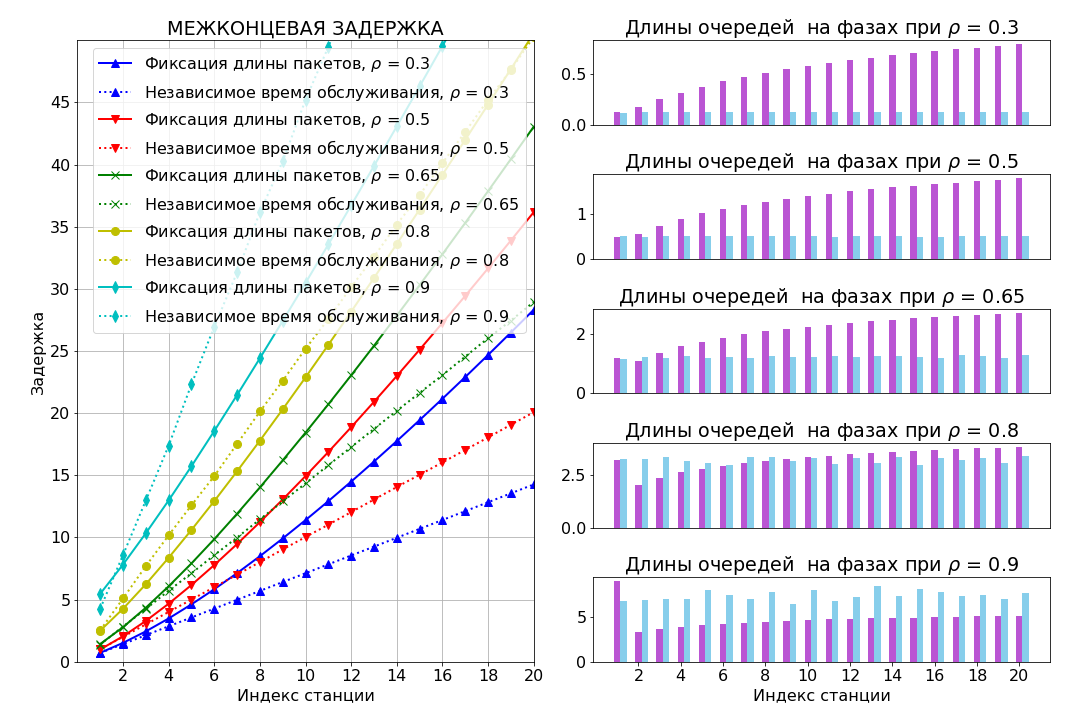
\includegraphics[width=0.8\textwidth]{sim20_model.png}
\caption{Задержки для случаев с независимой и зависимой функции распределения времени обслуживания}
\label{fig:sim20_model}
\end{figure}

\section{Модели прогноза времени межконцевой задеркжи с помощью методов машинного обучения}
\begin{figure}[h!]
    \centering
     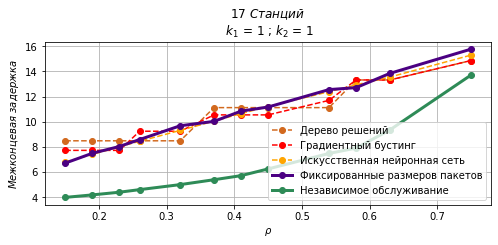
\includegraphics[width=0.8\textwidth]{17predict_model.png}
  \caption{Оценки времени межконцевых задержек для тандема размером 17}
  \label{fig:17predict_model}
\end{figure}

\section{Выводы по главе \cref{prediction_model}}


% \chapter{Математические модели синтеза топологии сети для охвата линейного участка в виде экстремальной задачи в комбинаторной форме}\label{chapter_combinatorial_model}

% Эффективным способом повышения технико-экономических показателей при проектировании \fixme{БШС} является оптимизация топологии сети, а именно решение задачи выбора оптимального набора станций из заданного избыточного множества и определение мест их размещения вдоль линейной контролируемой территории.
% Основным результатом работы, представленной в этой главе, является разработка итерационного метода выбора оптимальной топологии сети в процессе комплексного проектирования БШС. 
% Принципиальной особенностью предлагаемого метода, повышающей его эффективность, является то, что для рассмотрения на этапе моделирования предлагается не одно решения, а последовательности лучших решений задачи оптимизации топологии сети. Это позволяет с помощью разработанной итерационной процедуры выбирать на этапе моделирования лучшее решение среди тех решений по топологии, которые удовлетворяют требуемым характеристикам проектируемой БШС. 

% \section{Постановка задачи и ее формулировка в экстремальной комбинаторной форме}

% Пусть задано множество станций $S=\{s_j\}$ с параметрами $s_j=\{r_j,\{R_{jq} \},\mu_j, c_j \},j=1,...,m;q=1,...,m;j \neq q $. Здесь $r_j$ -- максимальный радиус покрытия станции, $\{R_{jq} \}$ -- множество максимальных радиусов связи между $j$-ой и $q$-ой базовой станции, $\mu_j$ - интенсивность времени обслуживания и $c_j$ -- стоимость станции.

% Задана максимальная допустимая стоимость размещенных станций $C$. 


% Задан отрезок $\alpha$ длиной $L$ с концами в точках $a_0$ и $a_{n+1}$. Внутри отрезка $\alpha = [a_0, a_{n+1}]$ задано множество возможных точек размещения станций множества $A=\{a_i \},i=1,...,n$ c координатами $l_i$.Точка $a_0$ имеет координату $l_0=0$, точка $a_{n+1}$ имеет координату $l_{n+1}=L$. На концах отрезка, в вершинах $a_0$ и $a_{n+1}$, стоят станции специального вида $s_0$ и $s_{m+1}$, соответственно, для которых радиусы покрытия, пропускные способности и стоимости не задаются. Радиусы связи задаются как $R_{0j}$ и $R_{(m+1)j}$, соответственно.
% Требуется разместить станции таким образом, чтобы максимизировать размер контролируемой ими территории (покрытие) отрезка $L$ при выполнении требования наличия связи каждой станции со станциями на концах отрезка (шлюзами) через систему размещенных станций при выполнении ограничений на время межконцевой задержки $T$ и суммарную стоимость размещенных станций $C$.
% Сформулируем задачу в виде экстремальной задачи на конечном множестве.

% \textit{Допустимой расстановкой станций} назовем такой возрастающий по величине координат $l_i$  набор пар $P = \{a_i, s_j\},a_i \in A,i \neq 0,i \neq n+1;s_j \in S$, для которого выполняются требования:

% % \begin{enumerate}
% % 	\item left connectivity: $\forall\;(a_i, s_j),\,1 \leq i \leq n,$ either $\exists (a_k, s_q):\:l_k < l_i $ 
% % 	and $l_i - l_k \leq \min \{R_j, R_q \},$ or $l_i - l_0 \leq R_j$;
% % 	\item right connectivity: $\forall\;(a_i, s_j),\,1 \leq i \leq n,$ either $\exists (a_t, s_g):\:l_t > l_i $ 
% % 	and $ l_t - l_i \leq \min \{R_j, R_g \}, $ or $ l_{n+1} - l_i \leq R_j$;	
% % 	\item $|P| = m$.
% % \end{enumerate}
% \begin{enumerate}
%     \item  для каждой пары $(a_i,s_j)$:
%         \begin{enumerate}
%             \item слева: либо найдется такая пара $(a_k,s_q)$, что, $l_i - l_k \leqslant R_{jq}$  и $l_i - l_k  \leqslant R_{qj}$, либо $l_i-l_0 \leqslant R_{j0}$ и $l_i - l_0 \leqslant R_{0j}$;
%             \item справа: либо найдется такая пара $(a_t,s_g)$, что, $l_t-l_i \leqslant R_{jq}$ и $l_t - l_i \leqslant R_{qj}$, либо $l_{n+1}-l_i \leqslant R_{j(m+1)}$ и $l_{n+1}-l_i \leqslant R_{(m+1)j}$. 
%         \end{enumerate}
% % - слева: либо найдется такая пара (a_k,s_q), что, l_i-l_k≤R_jq  и l_i-l_k  ≤R_qj, либо l_i-l_0≤R_j0 и l_i-l_0≤R_0j;
% % - справа: либо найдется такая пара (a_t,s_g), что, l_t-l_i≤R_jq и l_t-l_i  ≤R_qj, либо l_(n+1)-l_i≤R_(j(m+1)) и l_(n+1)-l_i≤R_((m+1)j). 
% Данное требование гарантирует, что любая станция может быть связана со станциями на концах отрезка либо через промежуточные станции, либо непосредственно;
%     \item в одной точке стоит не более одной станции;
%     \item сумма задержек по всем размещенным станциям меньше заданной величины $T$ – средней межконцевой задержки по времени по всей системе станций:
%     \begin{displaymath}
%         \label{eq:part3_e2e_delay}
%         \sum\limits_{j \in S_\sigma} \overline{T_j} \leqslant T,
%     \end{displaymath}
% где $S_\sigma$ – множество размещенных станций, $\overline{T_j}$ -- среднее время задержки на станции. Расчет задержек описан в параграфе \cref{part4_e2e_delay_section}
%     \item суммарная стоимость размещенных станций меньше заданного бюджетного ограничения  $C$.
% \end{enumerate}

% Каждой допустимой расстановке станций $P$ соответствует величина покрытия $z(P)$, определяемая как суммарная длина всех таких участков $\tau,\tau \subset \alpha$, что каждая точка этих 
% участков попадает в зону покрытия, по крайней мере, одной станции, входящей в набор пар $P$.

% Для удобства описании в дальнейшем алгоритмов введем понятие «недопокрытия» отрезка $\alpha$:

% \begin{displaymath}
%     f(P) = L - z(P)
% \end{displaymath} 

% Пусть $G$ -- множество всех допустимых расстановок $P$.
% Тогда мы можем сформулировать нашу задачу в следующей комбинаторной форме экстремальной задачи на конечном множестве. 

% \textbf{Задача 1.}

% Требуется найти такую допустимую расстановку  $P^*$, что
% \begin{equation}
%     \label{eq:part3_P}
%     P^* = \argmin \limits_{P \in G} f(P)
% \end{equation}

% Обозначим через $\Gamma$ все множество вариантов размещения станций (не обязательно допустимых) из множества $S$ на заданном множестве возможных мест их размещения.

% \section{Дерево ветвлений для перебора элементов в множестве \texorpdfstring{$\Gamma$}{Lg}}

% Опишем процедуру построения бинарного дерева поиска (дерева ветвлений) для полного перебора без повторений всех элементов множества $\Gamma$. Данная процедура будет использована в дальнейшем при построении дерева поиска в алгоритме МВиГ решения \textbf{задачи 1}.

% В дальнейшем будем предполагать, что в множестве $S$ станции упорядочены по не убыванию радиусов покрытия. 
% Описываемая процедура использует известный прием разбиения множества $G$ на подмножества с использованием некоторого параметра. Процесс формирования и последовательность исследования подмножеств обычно представляется с помощью дерева поиска, представляющего собой ориентированное от корня «дерева ветвлений», где каждому подмножеству соответствует вершина на дереве. Множеству $\Gamma$ соответствует корневая вершина. 

% \subsection{Параметр для разбиения множеств на подмножества}
% \textit{\textbf{Процедура 1.}}

% Пусть $G_0$, где нижний индекс – номер итерации, исходное множество $\Gamma$. На каждой итерации, начиная с итерации $\nu=0$, разбиваем текущее подмножество $G_\nu$ на два подмножества $G^1_\nu$ и $G^2_\nu$. При этом множество $G_\nu$ обычно называется «материнским», а множества $G^1_\nu$  и $G^2_\nu$  - «потомками» множества $G_\nu$ или дочерними узлами.

% В качестве параметра разбиения воспользуемся переменной $\pi_{ij}$, принимающей два значения 0 и 1:

% \begin{itemize}
%     \item $\pi_{ij}=1$, если наложено условие, что на месте $a_i$ расположена станция $s_j$;
%     \item $\pi_{ij} = 0$, если наложено условие, что на месте $a_i$ станция $s_j$  располагаться не будет.
% \end{itemize}

% В дальнейшем будем считать, что для множества $G^1_\nu$ задано условие $\pi_{ij}=1$, а для множества $G^2_\nu$  задано условие $\pi_{ij} = 0$.

% Очевидно, что

% \begin{equation}
%     \label{eq:part4_G_cup}
%     G^1_\nu \cup G^2_\nu = G_\nu;
% \end{equation}


% \begin{equation}
%     \label{eq:part4_G_cap}
%     G^1_\nu \cap G^2_\nu = \varnothing.
% \end{equation}

% Выбор переменной для разбиения на $\nu$-ой итерации

% На этапе разбиения любого множества $G_\nu$ все множество переменных $\Pi = \{\pi_{ij}\}$ можно разделить на три подмножества: множество $\Pi^+$ -- «фиксированные» переменные, для которых $\pi_{ij}=1$, множество $\Pi^-$ -- «запрещенные» переменные, для которых $\pi_{ij}=0$, и множество $\Pi^f$ -- «свободные» переменные, для которых значения на данной итерации еще не заданы.

% Правило выбора переменной для разбиения множества $G_\nu$. Для разбиения множества $G_\nu$ на данной итерации выбирается из множества $\Pi^f$ переменная c наименьшим индексом $j$ среди всех переменных с наименьшим индексом $i$. Таким образом сначала определяется незанятое место размещения $a_i$ с наименьшим номером (индексом $i$) и на нем размещается еще не размещенная станция $s_j$ с наименьшим номером (индексом $j$).

% \subsection{Движение по дереву ветвлений}

% После разбиения очередного подмножества $G_\nu$ два подмножества $G^1_\nu$  и $G^2_\nu$, последним на дереве ветвлений присваиваются порядковые индексы $G_{\nu+1}$ и $G_{\nu+2}$, соответственно.
% При формировании дерева ветвлений различаются два типа шагов: «прямой» шаг и «обратный» шаг. Прямой шаг -- это движение «в глубину» по той же ветви дерева, реализующее очередное разбиение множества $G_\nu$ на два потомка, и обратный шаг, реализующий переход от множества $G_\nu$  к одному из ранее сформированных подмножеств. Обратный шаг делается в том случае, когда либо получено множество $G_\nu$, состоящее из единственного элемента, либо множество $G_\nu$  при данном наборе значений переменных $\pi_{ij}$, выделяющих данное подмножество $G_\nu$ из множества $G_0$, пусто. В этих случаях соответствующая вершина дерева называется «закрытой».

% Для движения по дереву будем использовать правило \fixme{LIFO}. На основании этого правила прямые шаги будут выполняться до тех пор, пока не будет получена закрытая вершина. На дереве ветвлений это соответствует продолжению движения по той же ветви дерева. При этом из двух множеств $G^1_\nu$  и $G^2_\nu$ первым будет исследоваться на возможность закрытия соответствующей вершины множество $G^1_\nu$. Если вершина в результате проведенного исследования не будет закрыта, то из неё будет продолжено дальнейшее движение по той же ветви (выполнение прямого шага). Если вершина будет закрыта, то будет выполнен обратный шаг: для дальнейшего рассмотрения и продолжения движения будет выбрана незакрытая вершина с наибольшим порядковым номером $\nu$ среди всех висячих вершин дерева (последняя сформированная вершина из нерассмотренных). Процедура будет завершена, когда все вершины дерева будут закрыты.

% Заметим, что выполнение условий \cref{eq:part4_G_cup, eq:part4_G_cap} гарантирует, что в результате завершения работы \textit{\textbf{процедуры 1}} будут просмотрены все элементы множества $\Gamma$ без повторений. Эти же условия определяют фундаментальное свойство дерева ветвлений: на каждой итерации объединение множеств $G_\nu$ всех висячих вершин дерева дает исходное множество $G_0$ корневой вершины.


% \subsection{Алгоритм метода ветвей и границ} \label{BnB}
% Для построения алгоритма \fixme{МВиГ} для решения \textbf{задачи 1} с использованием \textit{\textbf{процедуры 1}} для построения дерева ветвлений нам достаточно разработать методы исследования вершин дерева на возможность их закрытия.
% В соответствии с техникой \fixme{МВиГ} закрытие вершины в результате исследования, соответствующего ей множества $G_\nu$ возможно в трех случаях.

% \underline{\textit{\textbf{Случай 1.}}} Множество $G_\nu$ -- пусто, т.е. доказано, что в множестве $G_\nu$ при данном наборе фиксированных и запрещенных переменных $\pi_{ij}$ нет ни одной допустимой расстановки $P$.

% \underline{\textit{\textbf{Случай 2.}}} Доказано, что в множестве $G_\nu$ не может быть допустимой расстановки P с меньшим значением целевой функции (1), чем у лучшей расстановки $\widehat{P}$ из уже найденных. Значение функции $f(\widehat{P})$ называется «рекордом», а расстановка $\widehat{P}$ -- «рекордным решением». В качестве начального рекорда принимается число заведомо большое искомого оптимального решения, например, $L$ – длина всего отрезка.

% \underline{\textit{\textbf{Случай 3.}}} Найдено оптимальное решение \textbf{задачи 1} на множестве $G_\nu$.
% Прежде чем рассмотреть эти три случая, запишем важное свойство любого множеств $G_\nu$, являющееся следствием принятого правила выбора свободной переменной для разбиения очередного множества $G_\nu$ при прямом шаге. 

% \textit{\textbf{Свойство 1.}} Пусть для исследуемого множества $G_\nu, \nu > 0$, точка $a_k$ -- это одно любое из мест, на которых уже размещены станция из множества $S$ в соответствии с набором фиксированных и запрещенных переменных $\pi_{ij}$, выделяющим данное множество из множества $G_0$. Тогда для всех мест «слева» от $a_k$, т.е. точек $a_i$, $i<k$, размещение станций уже определенно (при этом некоторые места могут быть пустыми).
% Перейдем непосредственно к исследованию \underline{\textit{\textbf{случаев 1 – 3}}}.

% \underline{\textit{\textbf{Случай 1.}}}

% Проверка текущего множества $G_\nu$ на пустоту состоит в установлении факта невозможности выполнения требований 1) – 4) введенных ранее при определении допустимой расстановки.

% Рассмотрим проверку условия выполнения требования 1) для множества $G_\nu, \nu > 0$. 

% Пусть множество $G_\nu$  образовано разбиением материнского множества при помощи переменной $\pi_{kt}=1$. Проверяем, что каждый из радиусов $R_{th}$ и $R_{ht}$, где $h$ – индекс станции, размещенной на ближайшей слева к точке $a_k$ точке $a_d$ больше расстояния $l_k-l_d$. Если ближайшая слева точка – это точка $a_0$ (левый конец отрезка $\alpha$), то делается проверка, для радиуса $R_{t0}$ и $R_{0t}$. 

% Если данное условие не выполняется, то множество $G_\nu$ недопустимо, соответствующая вершина закрывается и делается шаг обратного хода в соответствии с \textit{\textbf{процедурой 1}}. 

% Если множество $G_\nu$ образовано разбиением материнского множества при помощи переменной $\pi_{kt}=0$ и $a_d$ -- точка с наибольшим индексом, среди точек, на которых уже размещены станции (точки $a_0$, если размещенных станций нет), то надо проверить, что среди нераспределенных станций, без учета станции $s_t$, есть такая станция $s_q$ что расстояние между точками $a_k$ и $a_d$ не больше, чем $R_{qh}$ и $R_{hq}$. Если проверка отрицательна, то множество $G_\nu$ -- пусто, соответствующая этому множеству на дереве поиска вершина должна быть закрыта и выполняется шаг обратного хода в соответствии с  \textit{\textbf{процедурой 1}}.

% Требование 2) выполняется соответствующим выбором очередной станции для размещения, требования 3) и 4) выполняются непосредственным суммированием соответствующих параметров у размещенных станций.

% \underline{\textit{\textbf{Случай 2.}}}
% Построим оценку величины «недопокрытия» для множества $G_\nu$, полученного из материнского множества добавлением условия $\pi_{kt}=1$. Частичным «недопокрытием» назовем величину $\Delta(k,d,p,t)$, которая вычисляется по формуле:

% \begin{equation}\label{eq:part4_delta}
% \Delta(k,d,p,t) = max\{\left(a_{k} - a_{d} \right) - \left(r_{p} + r_{t} \right), 0\}.
% \end{equation}

% Частичное «недопокрытие» \cref{eq:part4_delta} определяется для любых двух точек $a_d$ и $a_k$,$k>d$, на которых расположены станции $s_p$ и $s_t$ при условии, что между этими точками нет других станций. Очевидно, что для любой расстановки $P$ «недопокрытие» $f(P)$ вычисляется как сумма всех «недопокрытий» $\Delta(k,d,p,t)$ между местами размещения станций, включая концы отрезка $\alpha$, на которых стоят станции особого типа $s_0$ и $s_{m+1}$.

% \begin{displaymath}
% W(G_\nu) \leq f(P), P \in G_\nu. 
% \end{displaymath}

% Если $W(G_\nu) \geq f(\widehat{P})$, то множество $G_\nu$ не может содержать расстановки лучше уже найденной расстановки $\widehat{P}$ соответствующая множеству $G_\nu$  вершина на дереве поиска должна быть закрыта и далее выполняется шаг обратного хода в соответствии с  \textit{\textbf{процедурой 1}}. 

% Построим оценку «недопокрытия» для множества $G_\nu$, полученного из материнского множества добавлением условия $\pi_{kt}=1$. Оценку будем искать в в
% иде суммы

% \begin{displaymath}
%     W\left(G_\nu\right) = w_1 + w_2. 
% \end{displaymath}

% Величина $w_1 \left(G_\nu \right)$ вычисляется как сумма все частичных «недопокрытий» слева от вершины $a_k$ и величины радиуса покрытия, размещаемой станций $r_t$. Оценку $w_2 \left(G_\nu \right)$ вычислим «для недопокрытия» справа на части $\beta$ до конца отрезка $\alpha$ (точки $a_{n+1}$). Данную оценку получим релаксацией условий, определяющих допустимую расстановку станций на участке $\beta$. Найдем такое подмножество $S_\beta$ множества станций $S$, состоящее из еще не размещенных станций и дающее минимальное «недопокрытие» на участке $\beta$ при выполнении только условий 2) – 4). Для этого сформулируем следующую задачу булевого программирования.

% \underline{\textit{\textbf{Задача 2.}}}
% \begin{displaymath}
%     z = |\beta| - \sum\limits_{x_j \in S_\beta} r_j x_j \rightarrow min.
% \end{displaymath}
% при условии:

% \begin{equation}\label{eq:part4_task2_cost}
%     \sum\limits_{x_j \in S_\beta} c_j x_j \leqslant C,
% \end{equation}

% \begin{equation}\label{eq:part4_task2_m}
%     \sum\limits_{x_j \in S_\beta} x_j \leqslant m,
% \end{equation}

% \begin{displaymath}
%     x_j \in \{0, 1\},
% \end{displaymath}
% где $|\beta|$ -- длина отрезка отрезка  $\beta$, $m$ -- число свободных мест для размещения станций на отрезке $\beta$.

% Очевидно, что эффективность использования оценки в методе ветвей и границ определяется точностью оценки и временем ее вычисления. \underline{\textit{\textbf{Задача 2}}} -- это задача ЦЛП, являющаяся труднорешаемой \cite{Gari}. На основании \underline{\textit{\textbf{задачи 2}}} можно получить две оценки менее точные, но имеющие более эффективные методы решения. Заметим, что при снятии ограничения \cref{eq:part4_task2_cost} или \cref{eq:part4_task2_m} \underline{\textit{\textbf{задача 2}}} представляет собой целочисленную задачу о ранце c эффективным псевдополиномиальным алгоритмом решения \cite{Gari}. При этом с точки зрения точности оценки, более перспективным представляется снятие ограничения \cref{eq:part4_task2_m}, так как на практике, обычно, число возможных мест размещения станций существенно меньше числа размещенных станций, полученного в результате решения задачи. Назовем задачу, полученную снятием ограничения \cref{eq:part4_task2_m}, \underline{\textit{\textbf{задачей 3}}}.

% \underline{\textit{\textbf{Задачу 2}}} при снятии условия целочисленности на переменные назовем \underline{\textit{\textbf{задачей 4}}}. \underline{\textit{\textbf{Задача 4}}} есть задача линейного программирования. Очевидно, что \underline{\textit{\textbf{задачи 3}}} и \underline{\textit{\textbf{задачи 4}}}, являясь оценками целевой функции решения \underline{\textit{\textbf{задачи 2}}}, могут служить оценками $w_2 (G_\nu)$. Результаты численного эксперимента с различными оценками вынесены в \fixme{приложение 2}.

% Если множество $G_\nu$ получено из материнского добавлением условия $\pi_{kt}=0$, то оценка $W(G_\nu)$ равна оценке материнского множества.

% \fixme{В приложении 1} приведены результаты вычислительного эксперимента, показывающего время решения \underline{\textit{\textbf{задач 2, 3, 4}}} и относительную точность \underline{\textit{\textbf{задачи 3 и 4}}} по отношению к \underline{\textit{\textbf{задаче 2}}}.

% Перейдем к рассмотрению \underline{\textit{\textbf{случая 3}}}. Рассматривается только для множеств $G_\nu$, состоящих из единственной расстановки $P$, для которой «недопокрытие» $f(P)$ вычисляется как сумма всех недопокрытий $\Delta(k,d,p,t)$ между местами, где размещены станций, включая концы отрезка $\alpha$, на которых стоят станции $s_0$ и $s_{m+1}$. 

% Если для найденной расстановки $P$ выполняются условия 1) – 4), которые для единственной расстановки легко проверяются, и

% \begin{equation}
%     \label{eq:part4_is_less_than_record}
%     f(P) < f(\widehat{P}),
% \end{equation}
% то $f(P)$ принимается за новый рекорд $f(\widehat{P})$, расстановка $P$ становиться новым рекордным решением $\widehat{P}$ и выполняется шаг обратного хода в соответствии с \textit{\textbf{Процедурой 1}}, если неравенство \cref{eq:part4_is_less_than_record} не выполняется, то рекорд остается прежним и выполняется шаг обратного хода.

% Работа алгоритма МВиГ заканчивается, когда все вершины дерева поиска закрыты, при этом решение задачи: 

% \begin{displaymath}
%     P^{*} = \widehat{P},  f(P^*) = f(\widehat{P}).
% \end{displaymath}

% \subsection{Построения последовательности топологий для итерационной процедуры моделирования \fixme{БШС}}

% В результате проектирования \fixme{БШС} надо найти ее оптимальную топологию среди всех топологий, для которых будут выполняться все требования к показателям, исследуемым и рассчитываемым на этапе моделировании сети. Для решения этой задачи воспользуемся идеей метода построения последовательности планов \cite{Emelichev}.

% Рассмотрим \textbf{задачу 1.}

% Требуется найти такую допустимую расстановку $P^*$, что

% \begin{displaymath}
%     f(P^*) = min \{f(P), P \in G \}.
% \end{displaymath}

% Построим для этой задачи последовательность $\Gamma = P^1, P^2, ... ,P^k$ допустимых расстановок (решений) множества $G$ для заданного $k$, где 
% \begin{align}
%     f(P^1) &= f(P^*), \nonumber  \\
%     f(P^2) &= extr\{ f(P), P \in G \ P^1 \}, \nonumber \\
%     ... \nonumber \\
%     f(P^k) &= extr\{ f(P), P \in G \ P^1 \cup P^2 \cup ... P^k \}, \nonumber 
% \end{align}

% В последовательности $\Gamma$ каждое решение не лучше предыдущего и не хуже последующего.

% Теперь воспользуемся следующей процедурой. Будем последовательно, начиная с первой расстановки, выполнять этап моделирования \fixme{БШС}. Очевидно, что как только мы получим расстановку, удовлетворяющую всем требованиям этапа моделирования, мы решим задачу нахождения оптимальной топологии среди всех топологий, для которых выполняются все требования к показателям, исследуемым и рассчитываемым на этапе моделировании сети. Действительно, для всех предыдущих расстановок эти условия не выполняются, а все последующие расстановки в последовательности $\Gamma$ не могут быть лучше по критерию $f(P)$.

% Обсудим вопрос как строить подобную последовательность на основании алгоритма \fixme{МВиГ}, описанного в параграфе \cref{BnB}. Заменив неравенство \cref{eq:part4_is_less_than_record} на нестрогое и записывая все рекорды, полученные в процессе работы алгоритма, мы, очевидно, получим последовательность расстановок, где каждая расстановка не хуже предыдущей и не лучше последующей. Для получения последовательности $\Gamma$ достаточно «перевернуть» полученную последовательность, где первый элемент станет последним.

% Недостатком такой процедуры является то, что для исследования на этапе моделирования будут отобраны только расстановки не хуже первого рекорда и среди них может не оказаться расстановки, удовлетворяющей критериям моделирования.
% Для расширения множества $\Gamma$ можно сделать следующее. Зададим условие. что в результате решения \textbf{задачи 1} мы хотим получить не только оптимальное решение, но и все решения не хуже оптимального на величину $d$. Для решения такого варианта задачи достаточно неравенство \cref{eq:part4_is_less_than_record} в алгоритме \fixme{МВиГ} заменить следующим неравенством 

% \begin{equation}
%     \label{eq:part4_is_less_than_record_d}
%     f(P) \leqslant f(\widehat{P}) + d,
% \end{equation}
% где $d = \varepsilon \cdot L > 0, \varepsilon$ -- заданное отклонение в процентах, и запоминать все рекорды, полученные в процессе решения задачи.

% На основании неравенства \cref{eq:part4_is_less_than_record_d} можно построить итерационную процедуру, увеличивая величину $d$, если при данном ее значении допустимого решения на этапе моделирования не найдено.
% В \fixme{приложение 2} представлены результаты численного примера.

% \subsection{Расчет межконцевой задержки}\label{part4_e2e_delay_section}

% Одной из основных характеристик проектируемой сети является ее межконцевая задержка. Рассмотрим беспроводную сеть как сеть массового обслуживания (СеМО) с кросс-трафиком и с узлами $M/M/1$. По теореме Бурке \cite{Burke1956} на выходе узла $M/M/1$, а значит на входе каждой последующей фазы тоже пуассоновский поток. Интенсивность на выходе каждой фазы равна суммарной интенсивности всех входящих потоков с интенсивностями $\lambda$.

% По формуле Литтла \cite{Little1961} можно рассчитать время задержки на фазе. Интенсивность времени обслуживания рассчитывается по формуле: 

% \begin{displaymath}
%     \mu_j = p_j / w,
% \end{displaymath}
% где: $p_j$ - пропускная спобоность $j$-ой станции, Мбит/с; $w$ - средний размер пакета, Мбит.

% Для каждой станции коэффициент загрузки равен:


% \begin{displaymath}
% \rho_j= \frac{\sum{\lambda}}{\mu_j} = \frac{q \cdot \lambda}{\mu_j} <1,
% \end{displaymath}

% где $q$ -- число входящих потоков. Условие $\rho_j<1$ является необходимым и достаточным условием существования стационарного режима функционирования \fixme{СеМО}.

% Тогда среднее время задержки по времени на каждой станции:

% \begin{displaymath}
%     \overline{T_j} = \frac{\rho_j}{1 - \rho_j} \cdot \frac{1}{q \cdot \lambda}.
% \end{displaymath}

% Тогда межконцевая задержки в сети равна

% \begin{equation}
%     \label{eq:end_to_end_delay}
%     T^{e2e}= \sum{\overline{T_j}}.
% \end{equation}

% \subsection{Выводы по Главе \cref{chapter_combinatorial_model}}

% В работе предложена методика проектирования беспроводной широкополосной сети для контроля линейной трассы с использованием итерационной процедуры построения последовательности лучших решений задачи выбора и размещения базовых станций при выполнении технологических условий на проектирование сети и ограничения на стоимость размещаемых станций. 

% Предложенная методика позволяет на этапе моделирования выбирать лучшее решение среди тех решений по выбору и размещению станций, которые удовлетворяют требованиям, предъявляемым к проектируемой сети.

% Процедура нахождения последовательности лучших решений задачи выбора и размещения базовых станций основана на разработанном алгоритме \fixme{МВиГ}.


% % First we shall build $W(G_0)$.

% % Since all the stations must be placed, then the maximum coverage of $\alpha$ is obtained in situations when  it would be possible to place all the stations without intersections of their coverage radiuses . Each station $s_j$ covers the segment of length 2$r_j$, therefore, a total non - coverage cannot exceed the value.

% % \begin{displaymath}
% % W\left(G_0\right) = \max{\left\{L-\sum_{j=1}^{m}{2r_j,0}\right\}}.                                                                                  
% % \end{displaymath}

% % Now we will define $W(G_\nu)$, $\nu > 0$ as the sum of partial sums $w_1$ and $w_2$. 

% % \begin{displaymath}
% % W\left(G_\nu\right) = w_1 + w_2.                                                                                  
% % \end{displaymath}

% % Suppose $G_\nu$ is obtained by splitting a parent set by setting the variable $\pi_{kt}$ = 1. Then $w_1$ is "non-coverage" of the segment from $a_0$ to $a_k$ while $w_2$ is non-coverage of the segment from $a_k$ to $a_{n+1}$.

% % The sum $w_1$ is calculated by formula (\ref{eq1}) by summing non-coverages between the places where stations have been placed already. 

% % The sum $w_2$ is calculated as

% % \begin{equation}\label{eq2}
% % w_2 = max\left\{\left(l_{n+1}-l_k\right)-\left(r_t+\sum_{j\in S_v}{2r_j}\right),0\right\},
% % \end{equation}
% % where $S_\nu$ is the set of unplaced stations. 

% % The formula (\ref{eq2}) is analogous to the formula (\ref{eq1}) except the fact, that it is applicable to the part of segment $\alpha$ which is to the right from the last place where any station has been placed.

% % If $\pi_{kt}$ = 0 the estimation $W(G_{\nu})$ remains unchanged after splitting.

% % \subsection{Case 3.}
% % In this case we review only sets $G_\nu$, which consist of a single placement $P$, and $f(P)$ is obtained as the sum of non-coverages $\Delta(k,d,p,t)$ between known places where  stations are placed.

% %  If for the given placement the inequality $f(P) < f(\widehat{P})$ takes place, then the placement $P$ becomes a new current best value $\widehat{P}$ and backward step is applied.
 
% % The branch and bound algorithm will stop when all the vertexes of the searching tree will be closed.
 
% % The solution is
% % \begin{displaymath}
% % P^{*} = \widehat{P},  \widehat{f}(P^*) = f(\widehat{P}).
% % \end{displaymath}

% % \section{Example 1}

% % \textit{Input data.}

% % The segment $\alpha$  with $L$ = 50, end points $a_0$  and  $a_4$  with coordinates $l_0$ = 0 and $l_4$= 50 is given. There are internal  points $a_1$, $a_2$, $a_3$ with coordinates $l_1$ = 20, $l_2$= 30, $l_3$=40.

% % The set of stations $S=\left\{s_j\right\}, j=1,2$  is given, where station $s_j$ has parameters: $r_1$ = 20, $R_1$ = 40; $r_2$ = 5, $R_2$ = 20. There are special stations $s_0$ and $s_4$, on the end points with $r_0$=$R_0$= 
% % $r_4$=$R_4$=0.

% % We have to find a feasible placement $P^*$, such that

% % \begin{displaymath}
% % P^* = \min \limits_{P \in G} f(P)
% % \end{displaymath}

% % The process of solving the problem is presented in the form of a binary search tree (see Fig.~\ref{fig2}).
 
% % The initial value of $f(\widehat{P})=L=50$, $G_0=G$.

% % The vertices of the tree indicated by $\emptyset$  correspond to the sets $G_\nu$ for which there are no feasible placements.

% % Two placements $P_1$ and $P_2$ were obtained as the current best solutions  with $f(P_1)=15$ and $f(P_2)=5$.

% % The optimal solution is $P^\ast=P_2,\ \ f\left(P^\ast\right)=f\left(P_2\right)=5$.

% % \begin{figure}
% % 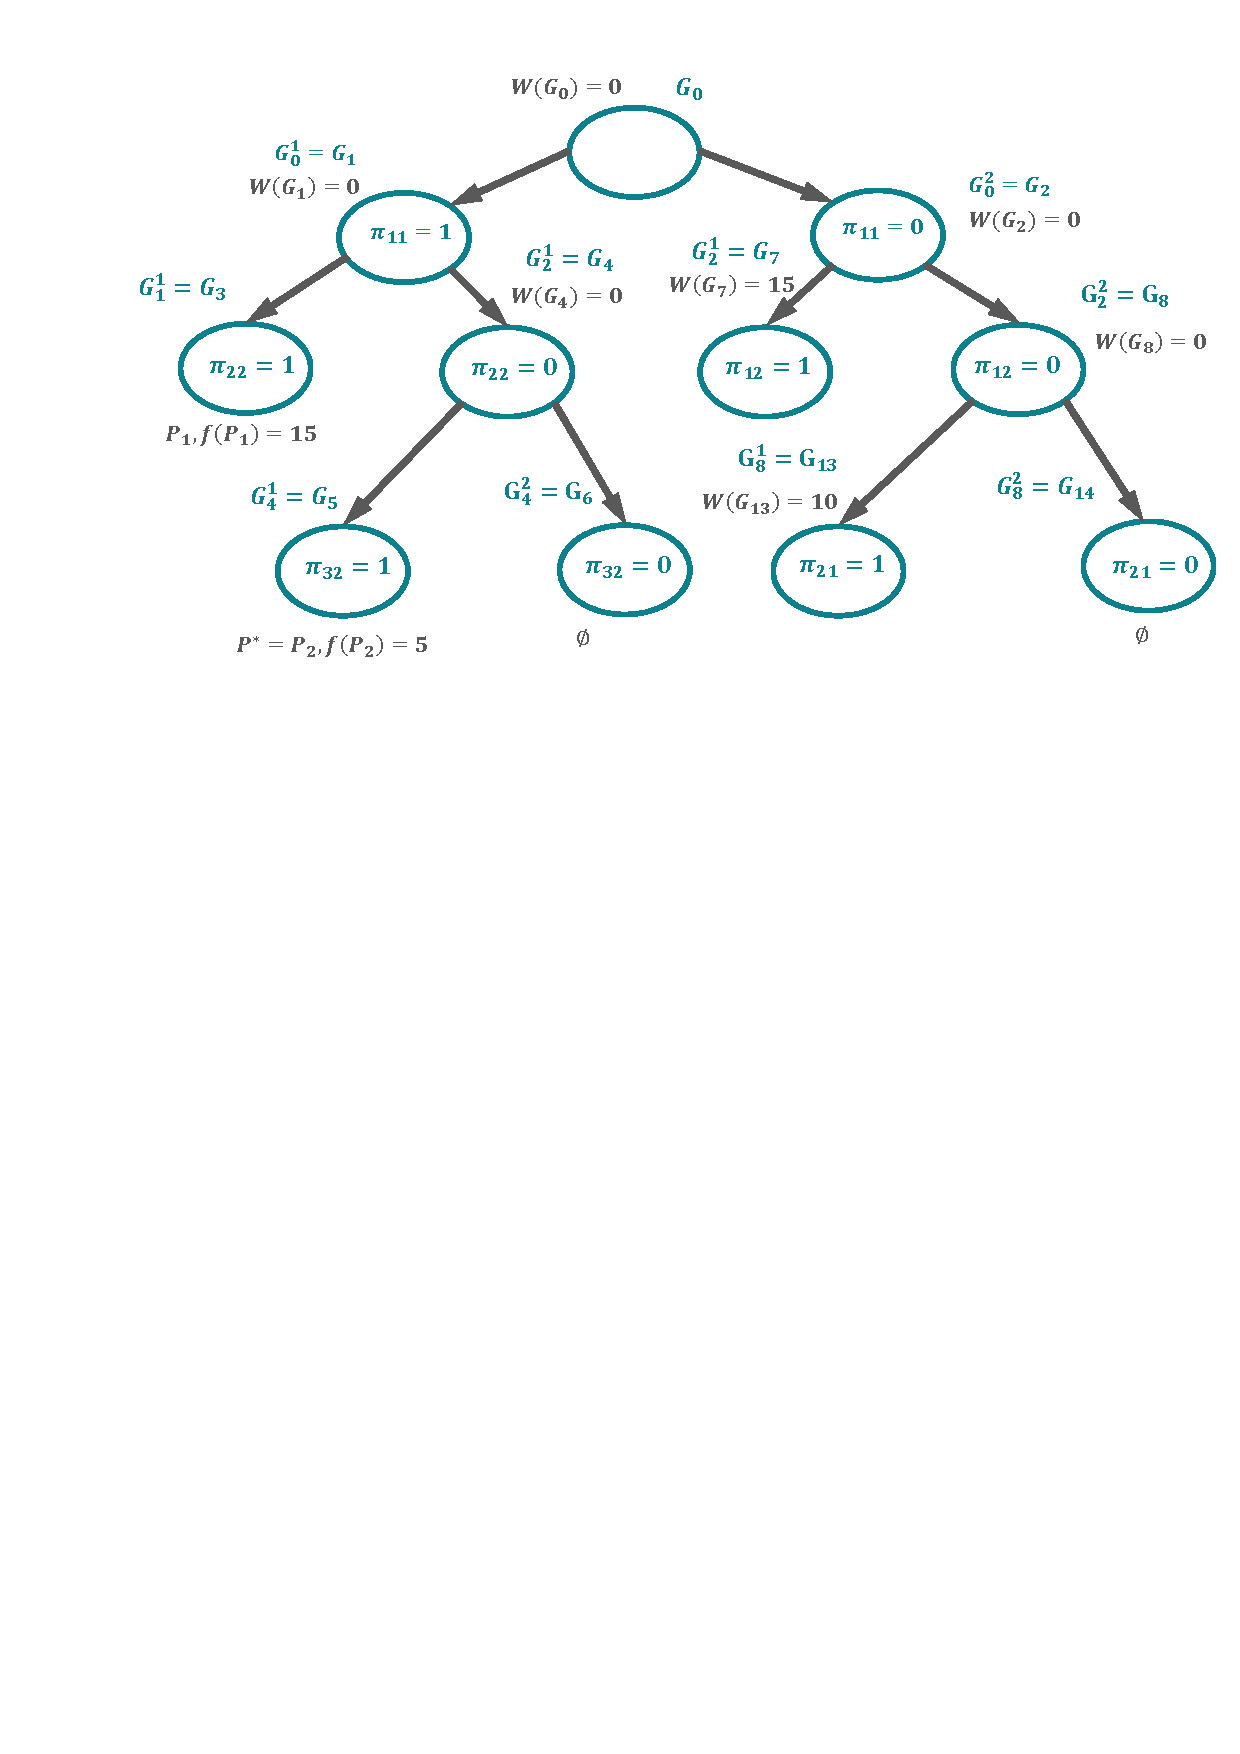
\includegraphics[width=\textwidth]{tree.pdf}
% % \caption{The search tree of branch and bound algorithm.} \label{fig2}
% % \end{figure}

% % \section{The statement of problem as a mixed – integer programming model}
% % Here we will formulate our placement problem in the form of a mixed – integer programming model. The description of problem is given in section 2.

% % Let us introduce binary variables $x_{ij}$ where $x_{ij}=1$ if a station $s_j$ is placed at point $a_i$ and $x_{ij}=0$ otherwise.

% % Let us introduce binary variables $e_i$ where $e_i$=1 if any station is placed at point $a_i$ and $e_i=0$ otherwise.

% % By definition

% % \begin{displaymath}
% % e_i=\sum_{j}^{m}{x_{ij}}, i=1,2,\ldots,n.
% % \end{displaymath}

% % We have $e_0$ = 1 and $e_{n+1}$ = 1 for the end points.

% % Let us formulate the following system of the problem constraints.

% % Each station must be placed in one and only one place

% % \begin{displaymath}
% % \sum_{i=1}^{n}{x_{ij}=1}, j=1,2,\ldots,m.
% % \end{displaymath}

% % At any point there can be no more than one station

% % \begin{displaymath}
% % \sum_{j=1}^{m}{x_{ij} \leq 1}, i=1,2,\ldots,m.
% % \end{displaymath}

% % We will introduce non-negative variables $y_i^+$  and  $y_i^-$ for points $a_i$, $i=0,1,2,..,n$, $n+1$.
% % Variables $y_i^+$ and  $y_i^-$  are the area sizes (right and left from point $a_i$) which are covered by station placed at point $a_i$.

% % Values of  variables $y_0^+$, $y_0^-$,$y_{n+1}^+$, $y_{n+1}^-$ equal 0.

% % The values of coverages are not greater than the coverage radius of the station located at $a_i$, and equal to 0 if is no station at $a_i$:

% % \begin{displaymath}
% % y_i^+\le\sum_{j=1}^{m}{x_{ij}r_j} ,i=1,2,\ldots,n,
% % \end{displaymath}

% % \begin{displaymath}
% % y_i^-\le\sum_{j=1}^{m}{x_{ij}r_j} ,i=1,2,\ldots,n.
% % \end{displaymath}

% % The total coverage area between any two points $a_i$ and $a_k$ on which the stations are located cannot exceed the distance between these points.

% % For  $i=1,\ldots,n$:

% % \begin{displaymath}
% % y_i^+ + y_k^- \le\frac{l_k - l_i}{2}\left(e_i + e_k\right)+\left(2 - e_i - e_k\right)L, k=i+1,\ldots,n+1,
% % \end{displaymath}

% % \begin{displaymath}
% % y_i^- + y_k^+  \le\frac{l_i - l_k}{2}\left(e_i + e_k\right)+\left(2 - e_i - e_k\right)L ,k=i-1,\ldots,0.
% % \end{displaymath}

% % 	This condition excludes the effect from intersections of station coverages when calculating the total coverage value for the entire segment $\alpha$.
	
% % 	According to the conditions of the problem, the station located at $a_i$ must be connected with at least one station on the left and one station on the right, including stations  at the end points $a_0$ and $a_{n+1}$.

% % 	We will introduce variables $z_{ijk}, i=1,2,\ldots,n$; $j=1,2,\ldots,m$; $k=1,2,\ldots,n$; $k\neq i$ to formulate this requirement where:

% % \begin{itemize}
% % 	\item $z_{ijk}=1$ if a station $s_j$ is located at point $a_i$ and connected with a station which is located at point  $a_k$;
% % 	\item $z_{ijk}=0$ otherwise.
% % \end{itemize}	
	
% % 	We will also introduce variables $z_{ij0}$ and $z_{ijn+1}$ where $z_{ij0}=1$ if a station $s_j$ is located at point $a_i$ and connected with a station $s_0$ which is located at point  $a_0$  and $z_{ij0} = 0$ otherwise; $z_{ijn+1}=1$ if a station $s_j$ is located at point $a_i$ and connected with a station $s_{n+1}$ which is located at point $a_{n+1}$  and $z_{ijn+1} = 0$ otherwise.

% % Stations must be at both points so that they can be connected: 

% % \begin{displaymath}
% % z_{ijk}\le e_i,  \forall i,j,k,
% % \end{displaymath}

% % \begin{displaymath}
% % z_{ijk}\le e_k, \forall i,j,k.
% % \end{displaymath}

% % The station $s_j$ which is located at $a_i$ must be connected with at least one station which is located right from $a_i$ and at least one station  which is located left from $a_i$

% % \begin{displaymath}
% % \sum_{k=i+1}^{n+1}{z_{ijk} \geq x_{ij}}, \forall i,j,
% % \end{displaymath}

% % \begin{displaymath}
% % \sum_{k=0}^{i-1}{z_{ijk} \geq x_{ij}}, \forall i,j.
% % \end{displaymath}

% % The communication radius $R_j$ of the station located at the point  $a_i$, must be no less than the distance to the point $a_k$, where there is a station with which it is connected:

% % \begin{displaymath}
% % z_{ijk\ }\left(R_j-\left(a_i-a_k\right)\right)\geq 0, k=i-1,\ldots,0, j=1,2,\ldots,m,  
% % \end{displaymath}

% % \begin{displaymath}
% % z_{ijk}\left(R_j-\left(a_k-a_i\right)\right)\geq 0, k=i+1,\ldots,n+1, j=1,2,\ldots,m. 
% % \end{displaymath}

% % Objective function

% % \begin{displaymath}
% % f=\sum_{i=1}^{n}{\left(y_i^++y_i^-\right)\rightarrow max} 
% % \end{displaymath}


% % \section{Numerical results}
% % The algorithms Branch and Bound (BnB) and brute-force algorithm (BF) were implemented using Python.
% % Table 1 shows the results of solving several problems for a different number of locations and a different number of stations using the B and B algorithm, the BF algorithm and the standard program for solving mixed – integer problem in the MATLAB package. We compare the number of vertices in the search trees so that the execution parameters of the algorithms do not depend on the speed of the machine and/or the quality the computer program. For each set of stations and set of placements   10 examples were computed with different numerical input data. For B and B and the MATLAB package the table shows the average execution parameters of the number of vertices in the search tree for each of the 10 examples.

% % \begin{table}
% % \caption{The results of solving problems.}\label{tab1}
% % \begin{tabular}{|l|l|l|l|l|}
% % \hline
% % {\bfseries Places} & {\bfseries Stations} &	{\bfseries BF}& {\bfseries BnB} & {\bfseries MILP} \\ 
% % \hline
% % 7 &		5 &	17550  &	933 &		753\\
% % 9 &		5 &	71090  &	6478 &		2669\\
% % 10 &	5 &	126180 &	1041 &		8551\\
% % 12 &	6 &	No &		8294 &		38569\\
% % 13 & 	6 &	No &		18485 &		30369\\
% % \hline
% % \end{tabular}
% % \end{table}

% % \textit {The numerical results. “No” means the problem was not solved after 3 hours}. 

% % \section{Conclusion}

% % In this  paper the problem of finding optimal location for the  given set of base stations in wireless network with linear topology was analyzed. The problem has been formulated as an  extremal combinatorial problem and also as mixed – integer linear programming model.  The branch and bound algorithm for solving the problem in combinatorial form was developed. The results of the computer experiment show that the branch and bound algorithm is more effective than the brute-force algorithm and using of the branch and bound algorithm also more effective than to solve the problem represented as a mixed–integer programming model.
